\documentclass[10pt,a4paper]{article}
% Shared layout for the two reading guides (vademecum) that accompany the decks.
\usepackage[T1]{fontenc}
\usepackage[utf8]{inputenc}
\usepackage[english]{babel}
\usepackage{mathpazo}
\usepackage{amsmath,amssymb,bm,booktabs,array,graphicx,microtype,xcolor}
\usepackage[a4paper,left=14mm,right=14mm,top=11mm,bottom=14mm]{geometry}
\usepackage{titlesec,enumitem,siunitx}
\usepackage[most]{tcolorbox}
\tcbuselibrary{raster}
\usepackage[colorlinks=true,urlcolor=accent,linkcolor=accent]{hyperref}
\sisetup{group-separator={,},group-minimum-digits=4}
\definecolor{pisablue}{RGB}{74,96,121}
\definecolor{pisablight}{RGB}{192,206,220}
\definecolor{accent}{RGB}{26,118,179}
\definecolor{expert}{HTML}{C98A1E}
\definecolor{muted}{HTML}{666666}
\titleformat{\section}{\color{pisablue}\bfseries\normalsize}{\thesection}{.6em}{}
\titlespacing*{\section}{0pt}{1.6ex plus .4ex}{.5ex}
\titleformat{\subsection}[runin]{\color{pisablue}\bfseries\small}{}{0pt}{}[.]
\titlespacing*{\subsection}{0pt}{.7ex}{.5em}
\setlist{nosep,leftmargin=1.2em,topsep=.2ex}
\setlength{\parindent}{0pt}
\setlength{\parskip}{.45ex}
\pagestyle{plain}
\newtcolorbox{summarybox}{enhanced,colback=pisablight!22,colframe=pisablue!60,boxrule=.4pt,arc=0pt,left=5pt,right=5pt,top=3pt,bottom=3pt,fontupper=\small}
\newtcolorbox{paperbox}[1][]{enhanced,colback=pisablight!18,colframe=pisablue!55,boxrule=.4pt,arc=0pt,left=5pt,right=5pt,top=2pt,bottom=3pt,fontupper=\small,
 title={In the paper#1},fonttitle=\bfseries\small,coltitle=pisablue,colbacktitle=pisablight!18,titlerule=0pt,toptitle=2pt,bottomtitle=0pt}
\newtcolorbox{ideabox}{enhanced,colback=expert!8,colframe=expert,boxrule=.5pt,arc=0pt,left=5pt,right=5pt,top=2pt,bottom=3pt,fontupper=\small,
 title={Proposals, not in the paper},fonttitle=\bfseries\small,coltitle=expert!70!black,colbacktitle=expert!8,titlerule=0pt,toptitle=2pt,bottomtitle=0pt}
% \vademecumheader{title}{authors}{journal}{doi, URL-encoded}{doi as printed}{companion deck}
\newcommand{\vademecumheader}[6]{%
 {\color{pisablue}\large\bfseries #1\par}\vspace{.6ex}
 {\small #2\enspace\textperiodcentered\enspace #3\par}
 {\footnotesize\href{https://doi.org/#4}{doi:#5}\par}
 {\footnotesize\color{muted} Reading guide by Matteo Di Sante for the paper review; companion deck: #6. Equation, figure and section numbers are those of the paper.\par}\vspace{.8ex}}
\newcommand{\ours}{{\color{expert!70!black}\bfseries[ours]}}

\hypersetup{pdftitle={Reading guide: Arakawa and Schubert (1974)},pdfauthor={Matteo Di Sante}}
\newcommand{\MB}{\mathcal M_B}

\begin{document}
\vademecumheader{Interaction of a cumulus cloud ensemble with the large-scale environment, Part I}
{A. Arakawa, W.\,H. Schubert}
{J. Atmos. Sci. \textbf{31}, 674--701 (1974)}
{10.1175/1520-0469(1974)031\%3C0674:IOACCE\%3E2.0.CO;2}
{10.1175/1520-0469(1974)031<0674:IOACCE>2.0.CO;2}
{\texttt{arakawa-schubert1974.pdf} (10 slides)}

\begin{summarybox}
\textbf{In brief.} A closed theory of how an ensemble of cumulus clouds and the slowly varying large-scale environment, including the subcloud mixed layer, control each other; it became the Arakawa--Schubert convection scheme. (i) Clouds change the environment only through their total mass flux $M_c(z)$, which drives compensating subsidence, their detrainment $D(z)$, and the liquid water $\hat l(z)$ they detrain. (ii) The ensemble is split into sub-ensembles of entraining plumes labelled by their fractional entrainment rate $\lambda$; given the environment, each type's profile and top follow, and the only unknown is the cloud-base mass-flux distribution $\MB(\lambda)$. (iii) The mixed-layer depth $z_B$ is prognostic and is itself a control. (iv) The \emph{cloud work function} $A(\lambda)$, the kinetic energy generated per unit mass flux, depends only on the environment. (v) \emph{Quasi-equilibrium}: clouds remove $A$ in $\tau_{ADJ}\sim10^3$--$10^4$ s, much faster than the large scale creates it ($\tau_{LS}\gtrsim10^5$ s), so the cloud stabilization balances the large-scale forcing. This gives a Fredholm integral equation of the first kind for $\MB(\lambda)\geq0$, supported by tropical data.
\end{summarybox}

\section{Context (Section 1)}
Clouds in a large-scale disturbance have much smaller space and time scales, so their collective influence, not each cloud, can be predicted: cumulus parameterization. Its need became clear from the failure of early theories of tropical cyclones. CISK (Charney \& Eliassen 1964; Ooyama 1964), in which cumulus heating and the cyclone cooperate, used simple parameterizations that gave insight and some success, but were too crude in general; later schemes relied on empiricism and intuition, without a framework for the two-way interaction. There was agreement on how an existing ensemble changes the environment: detrainment cools and moistens, cumulus-induced subsidence warms and dries (Yanai et al.\ 1973, who also showed that shallow and deep clouds must coexist to close the tropical budgets; a single cloud type in the early UCLA GCM gave a too dry lower troposphere). Ooyama (1971) allowed clouds of different sizes, as non-interacting bubbles from below, and reduced the problem to a ``dispatcher function'' for bubble generation, which he left open. This paper closes the theory; the control is a destabilization by large-scale processes above and within the mixed layer, and the closure is the quasi-equilibrium of the cloud work function (Arakawa 1969).

\section{How the ensemble changes the environment (Sections 2--3)}
\subsection{Setup} A unit horizontal area between cloud base and the highest top contains many clouds but is a fraction of the large-scale disturbance. Continuity is quasi-Boussinesq, $\nabla\cdot(\rho\mathbf v)+\partial_z(\rho w)=0$ with $\rho(z)$. Cloud $i$ covers $\sigma_i(z,t)$ with mass flux $M_i=\rho\sigma_iw_i$; entrainment $E_i=\partial_zM_i+\rho\partial_t\sigma_i$ where positive, detrainment $D_i$ where it is negative (Eqs.\ 3--4), so $E-D=\partial_zM_c+\rho\partial_t\sigma_c$ with $M_c=\sum_iM_i$ and $\sigma_c=\sum_i\sigma_i$. The environment mass flux is $\tilde M=\rho\bar w-M_c$: with intense convection $M_c>\rho\bar w$ and the air between clouds subsides. Variables: dry static energy $s=c_pT+gz$ (conserved in dry adiabatic motion), moist static energy $h=s+Lq$ (conserved in moist adiabatic motion), mixing ratio $q$.

\subsection{Approximations} (a) $\sigma_c\ll1$ (Eq.\ 18), supported by observations (Malkus et al.\ 1961) and theory: conditional instability favours narrow rising areas (Bjerknes 1938), and heat transport is most efficient when the rising area is a few percent (Asai \& Kasahara 1967). Then $\bar s\approx\tilde s$ (23) and, unless the environment is extremely dry, $\bar q\approx\tilde q$ (25): predicting the environment is predicting the large scale. (b) Horizontal eddy transports by clouds across the area boundary are negligible (26--28). (c) No storage of mass, energy or water in the ensemble (37--39). (d) Detrained liquid water evaporates at the detrainment level (40), valid for droplets, not raindrops.

\subsection{Individual clouds} Budgets of mass, $s$, $q$ and liquid water $l$ are written for the entrainment layer (43--46) and for a detrainment layer (47--50), with condensation $C_i$ and conversion to rain $R_i$. Cloud air is saturated; neglecting pressure differences, $s_i-\bar s\approx(h_i-\bar h^*)/(1+\gamma)$ with $\gamma=(L/c_p)(\partial\bar q^*/\partial T)_p$ (54--57); $\partial\bar h^*/\partial z\gtrless0$ marks moist-adiabatically stable or unstable lapse rates. A growing cloud entrains at all levels, including its top; once the top stops rising it detrains in a thin layer, at about the level of vanishing buoyancy. Buoyancy uses the virtual static energy $s_v=s+c_p\bar T(\delta q-l)$, $\delta=0.608$ (58). At that level all clouds share a liquid water $\hat l(z)$ (62), and vanishing buoyancy reads $h_i=\hat h^*$, with $\hat h^*=\bar h^*-\frac{(1+\gamma)L\epsilon}{1+\gamma\epsilon\delta}[\delta(\bar q^*-\bar q)-\hat l]$, $\epsilon=c_p\bar T/L$ (63--64).

\subsection{Result: the prediction equations (74)--(75)}
\[
\rho\frac{\partial\bar s}{\partial t}=D(\hat s-\bar s-L\hat l)+M_c\frac{\partial\bar s}{\partial z}-\rho\bar{\mathbf v}\cdot\nabla\bar s-\rho\bar w\frac{\partial\bar s}{\partial z}+\bar Q_R,\qquad
\rho\frac{\partial\bar q}{\partial t}=D(\hat q^*+\hat l-\bar q)+M_c\frac{\partial\bar q}{\partial z}-\rho\bar{\mathbf v}\cdot\nabla\bar q-\rho\bar w\frac{\partial\bar q}{\partial z},
\]
with $\hat s$, $\hat q^*$ the detrainment values (72--73) and $\bar Q_R$ the radiation, including that of the clouds. The first term is detrainment: cooling and moistening by the evaporation of detrained water. The second is cumulus-induced subsidence: warming ($\partial_z\bar s>0$) and drying ($\partial_z\bar q<0$). The latent heat released inside the clouds does not warm the environment directly: it keeps the clouds buoyant against entrainment and adiabatic cooling, so it maintains $M_c$ and thus the subsidence warming, whose vertical distribution can differ greatly from that of condensation (first used by Arakawa 1969). The same equations follow from total-area budgets (31--36), where the cumulus eddy fluxes are $\overline{\rho ws}-\rho\bar w\bar s\approx\sum_iM_i(s_i-\bar s)$ (35). \emph{The parameterization problem reduces to $M_c(z)$, $D(z)$ and $\hat l(z)$} (plus cloud radiation).

\section{Spectral representation of the ensemble (Section 4)}
\subsection{Cloud types} Finding $D(z)$ means finding the mass flux of the clouds that lose buoyancy at each level. Assume one parameter $\lambda$ characterizes a cloud type, with detrainment (top) level $z_D(\lambda)$ decreasing with $\lambda$ and inverse $\lambda_D(z)$. With the sub-ensemble mass flux $\mathcal M(z,\lambda)\,d\lambda=\sum_{\lambda_i\in(\lambda,\lambda+d\lambda)}M_i(z)$,
\[
M_c(z)=\int_0^{\lambda_D(z)}\mathcal M(z,\lambda)\,d\lambda,\qquad D(z)=-\mathcal M\big(z,\lambda_D(z)\big)\frac{d\lambda_D}{dz},\qquad \mathcal M(z,\lambda)=\MB(\lambda)\,\eta(z,\lambda),\ \ \eta(z_B,\lambda)=1 .
\]
The base $z_B$ is the top of the subcloud mixed layer, somewhat below cloud base $z_C$; there the mass flux is that of the updrafts \emph{associated with} the clouds, not in them. Sub-ensemble budgets give $\partial_z\eta=\mu\eta$ and $\partial_zh_c=-\mu(h_c-\bar h)$, where $\mu=\eta^{-1}\partial_z\eta$ is the fractional entrainment rate (83--89). If $\eta$ is known, $h_c$ follows by integration, $q_c$ from saturation (90), $l$ with a rain parameterization $r(z,\lambda)$, and the top from vanishing buoyancy, $h_c[z_D(\lambda),\lambda]=\hat h^*[z_D(\lambda)]$ (92). Members of a sub-ensemble are at random phases of their life cycle, so $\eta$ is the lifetime-averaged profile of a single cloud.

\subsection{Choice of $\lambda$} Simpson's one-dimensional tower model, widely tested against observations, has $\mu=2\alpha/R$ (94), with $R$ the tower radius and $\alpha$ an entrainment constant. \emph{A radius constant with height in the Lagrangian sense fits observations better than horizontally expanding thermals or starting plumes (Simpson et al.\ 1965).} The authors assume that the fractional entrainment rate \emph{of the time-averaged mass flux} is constant with height, and use it as $\lambda$: the cloud need not be a steady jet and may be a sequence of active elements with negligible horizontal expansion below the level of vanishing buoyancy. Large $\lambda$ means small clouds. Then
\[
\partial_z\eta=\lambda\eta\ \Rightarrow\ \eta(z,\lambda)=e^{\lambda(z-z_B)}\ \ (z_B\leq z\leq z_D(\lambda)),\qquad
h_c(z,\lambda)=\frac{1}{\eta(z,\lambda)}\Big[h_c(z_B,\lambda)+\lambda\int_{z_B}^z\eta(z',\lambda)\,\bar h(z')\,dz'\Big],
\]
and above condensation $s_c-\bar s=(h_c-\bar h^*)/(1+\gamma)$ (98). With Jordan's (1958) mean hurricane-season sounding, $p_B=950$ mb and $h_M=82$ cal\,g$^{-1}$ (Figs.\ 6--8): larger $\lambda$ are diluted faster by the low-$\bar h$ mid-troposphere and detrain lower; $\lambda$ from 0 to about 20\% km$^{-1}$ spans tops from near 150 mb to the lower troposphere. What remains unknown is $z_B$, the cloud-base properties and, above all, $\MB(\lambda)$, the counterpart of Ooyama's dispatcher function.

\section{The subcloud mixed layer (Section 5)}
Observations (Bunker et al.\ 1949; Malkus 1958) show a mixed layer from the sea surface to about 200 m below cloud base, with constant $\theta$ and $q$, hence $s$ and $h$, and a thin transition layer above it where $\theta$ rises and $q$ drops. Only unsaturated mixed layers are treated (saturated ones: Randall \& Arakawa 1974). The transition layer is a discontinuity at $z_B$ (as in Ball 1960; Lilly 1968; Deardorff 1972; Betts 1973a) with jumps $\Delta s$, $\Delta q$, $\Delta h=\Delta s+L\Delta q$; typically $L\Delta q$ dominates and $\Delta h<0$, so updrafts prefer to start in the mixed layer, the only case treated. Mixed-layer budgets (103--109) with turbulent fluxes $F_s$, $F_q$, and flux continuity across the transition layer with $M_B=\int_0^{\lambda_{\max}}\MB\,d\lambda$ (110--118), are closed with Lilly's relation $(F_{sv})_B=-k(F_{sv})_0$ between the fluxes of virtual static energy $F_{sv}=F_s+c_p\bar T\delta F_q$ at the top and at the surface (119--120). The coefficient $k\in[0,1]$ spans no to maximal entrainment; $k\approx0.10$ from tank experiments (Deardorff et al.\ 1969), 0.25 (Betts 1973a). The depth then obeys
\[
\rho_B\frac{Dz_B}{Dt}=-(M_B-\rho_B\bar w_B)+\frac{k}{\Delta s_v}(F_{sv})_0,\qquad \Delta s_v=\Delta s+c_p\bar T\delta\Delta q>0\ \ \text{(dry stability)},
\]
with prognostic $s_M$, $q_M$, $h_M$ (124--127) and an approximation for small $\Delta s_v$ (128; Appendix A). Without clouds the layer deepens when $\rho_B\bar w_B+k(F_{sv})_0/\Delta s_v>0$. Cumulus-induced subsidence counteracts the deepening and can make the layer shallower; but a shallow layer supplies a smaller share of the air entering the clouds, and more comes from the drier air above, which is unfavourable for an active ensemble. So the variable depth is part of the mechanism controlling the total mass flux. Unlike Betts (1973a), $z_B$ is not set equal to $z_C$. Clouds start with mixed-layer properties, $s_c(z_B,\lambda)=s_M$, $q_c=q_M$, $h_c=h_M$ (129--131): the layer's primary role is to supply moisture and energy. Some perturbation of the mixed layer is needed to trigger a cloud, and it could act on $z_B$ rather than on $s_M$ or $q_M$.

\section{The cloud work function (Section 6)}
The conceptual difficulty is how, if at all, the large scale controls the spectrum $\MB(\lambda)$. Only $\MB$, not the number distribution of clouds, is needed. The kinetic energy of type-$\lambda$ clouds obeys
\[
\frac{d\mathcal K(\lambda)}{dt}=A(\lambda)\MB(\lambda)-\mathcal D(\lambda),\qquad
A(\lambda)=\int_{z_B}^{z_D(\lambda)}\frac{g}{c_p\bar T(z)}\,\eta(z,\lambda)\,\big[s_{vc}(z,\lambda)-\bar s_v(z)\big]\,dz ,
\]
valid for 2D or 3D convection, with mechanical interaction with the environmental shear and with other cloud types neglected. $A$ is the kinetic energy generated per unit cloud-base mass flux, an integral of buoyancy weighted by $\eta$. Since the buoyancy and the top of each type are fixed by the environment (134--135), \emph{$A(\lambda)$ is a property of the environment, including the mixed layer, and the only one that can influence kinetic-energy generation by type $\lambda$}. For $z_C=z_B$ it becomes (139): buoyancy at cloud base, $\rho\beta[h_M-\bar h^*(z_B+)]$, plus conditional instability, $-\partial_z\bar h^*$, reduced by a term $\lambda(\bar h-\bar h^*)$ that is negative in an unsaturated environment. Non-entraining clouds ($\lambda=0$) are insensitive to humidity above cloud base; entraining ones also need a moist environment. $A(\lambda)>0$ is a generalized, cloud-type-dependent criterion for moist convective instability, and $A=0$ for all $\lambda$ is a neutral environment. It is not sufficient: generation also needs $\MB>0$ and a trigger. \ours{} For $\lambda=0$, $A$ is close to what is now called CAPE.

Its tendency has cloud terms, linear in $\MB$ through $M_c$, $D$ and $M_B$, and large-scale terms:
\[
\frac{dA(\lambda)}{dt}=\int_0^{\lambda_{\max}}K(\lambda,\lambda')\,\MB(\lambda')\,d\lambda'+F(\lambda),\qquad F=F_C+F_M,\qquad K=K_V+K_D+K_M .
\]
$F>0$ destabilizes: $F_C$, from the cloud-layer equations, is dominated by cooling above the mixed layer, typically by large-scale ascent; $F_M$ includes mixed-layer deepening by large-scale ascent at $z_B$ and the surface flux of virtual static energy. $K$ is typically negative: $K\MB$ is the stabilization of type $\lambda$ by type $\lambda'$. The vertical mass-flux kernel $K_V$ mostly represents warming by subsidence induced by $\lambda'$ and is nearly symmetric (Fig.\ 11). The detrainment kernel $K_D$ vanishes for $\lambda'<\lambda$ and is nearly always positive for $\lambda'>\lambda$: shallower clouds increase the work function of deeper ones by moistening and evaporatively cooling their environment (Fig.\ 12). The mixed-layer kernel $K_M$ carries the effect of $z_B$. Explicit forms, from the time derivative of (133), fill Appendix B.

\section{Quasi-equilibrium and closure (Section 7)}
\subsection{Why the large scale controls $\MB$} In one-dimensional cloud models the upper cloud cannot affect cloud-base conditions, so subcloud processes alone would set $\MB$. In models with more dimensions only the first cloud needs an impulse; later cloud-base conditions are part of the solution. \emph{Small turbulent perturbations in the mixed layer are unlikely to trigger new clouds if $z_B$ is well below the condensation level; new clouds need stronger impulses, possibly from downdrafts of neighbouring clouds, or form in the wake of a preceding cloud, whose solenoidal circulation $A(\lambda)$ measures.} At $z_B$, $\MB(\lambda)\,d\lambda=\mathcal N(\lambda)\,d\lambda\,\mathrm m_B(\lambda)/\tau(\lambda)$ (145), with population $\mathcal N$, lifetime $\tau$ and lifetime-integrated single-cloud mass flux $\mathrm m_B$; $\mathcal N/\tau$ is Ooyama's dispatcher function. $\mathrm m_B$ is sensitive to cloud microphysics (Ogura \& Takahashi 1971), and ensemble simulations did not exist, so the three are not determined separately.

\subsection{Adjustment} Start with $A>0$, no forcing and a trigger: clouds grow, warm and dry the environment and thin the mixed layer, so $A$ decays to a neutral state in the adjustment time $\tau_{ADJ}$. With forcing, the system tends instead to an equilibrium $dA/dt=0$ where cloud and large-scale terms balance. If the forcing changes on $\tau_{LS}\gg\tau_{ADJ}$, the ensemble follows a sequence of equilibria set by the current forcing: the \emph{quasi-equilibrium assumption}, also an assumption on parameterizability. Orders of magnitude: $|[dA/dt]_C|\sim A/\tau_{ADJ}$ and $|dA/dt|\lesssim A/\tau_{LS}$, so $|dA/dt|\lesssim(\tau_{ADJ}/\tau_{LS})|[dA/dt]_C|$ (146--149). With cloud excess temperatures of a few degrees, $A\sim(10^{-1}\,\mathrm{m\,s^{-2}})H_c$; with $N^2\sim10^{-4}$ s$^{-2}$ and $\sigma_cw_c\sim0.1$--1 m\,s$^{-1}$, $[dA/dt]_C\sim(10^{-4}$--$10^{-5}\,\mathrm{m\,s^{-3}})H_c$; hence $\tau_{ADJ}\sim10^3$--$10^4$ s, one to two orders below $\tau_{LS}\gtrsim10^5$ s. The analogy is quasi-geostrophic balance.

\subsection{Closure} Dropping $dA/dt$,
\[
\int_0^{\lambda_{\max}}K(\lambda,\lambda')\,\MB(\lambda')\,d\lambda'+F(\lambda)=0\ \ \text{where}\ \MB(\lambda)>0,\qquad \int_0^{\lambda_{\max}}K\,\MB\,d\lambda'+F<0\ \ \text{where}\ \MB(\lambda)=0,
\]
a Fredholm integral equation of the first kind with a positivity constraint (150, 158); types with $A\leq0$ or unable to increase their own $A$ are absent. $A$ need not be constant: it is small, $A\sim\tau_{ADJ}[dA/dt]_{LS}$ (151), so quasi-equilibria are \emph{quasi-neutral} states. The value of $\tau_{ADJ}$ does not enter. An iterative solution method is in Part II (announced as Schubert \& Arakawa).

\subsection{Observational check (Figs.\ 13--14)} With the Marshall Islands data of Yanai et al.\ (1973), the observed $dA/dt$ for $\lambda=8$ and 16\% km$^{-1}$ scatters around zero while $F_C$ ranges up to about 1.5 cal\,g$^{-1}$\,day$^{-1}$, far from the no-cloud line $dA/dt=F_C$. $F_M$ could not be computed from conventional data; a rough estimate makes it considerably smaller than $F_C$. Mixed-layer top and cloud base were placed at 950 mb, with zero cloud-base buoyancy. At Eniwetok (May 1956, $\lambda=8\%$ km$^{-1}$), $A=I_1-I_2$ with $I_1$ depending on temperature and moisture and $I_2$ on temperature only (155--157): both vary by about 20 cal\,g$^{-1}$ while $A$ stays small and positive, a constraint that couples temperature and moisture changes.

\section{Conclusions and applications (Section 8)}
In models only $[dA/dt]_{LS}\Delta t$, the change of $A$ over a time step due to large-scale processes, is needed: solve for $\MB\Delta t$ and let the cloud terms bring $A$ back to zero, formally like moist convective adjustment (Manabe et al.\ 1965) but with explicit adjustment and implicit forcing. With an explicit $F$, the theory generalizes Charney \& Eliassen (1964), Ooyama (1964) and Kuo (1965), whose forcing was frictional or moisture convergence, adding advection, surface fluxes and radiation. Uses by 1974: diagnostic mass-flux distributions from observations (Ogura \& Cho 1973; Nitta 1974), the UCLA GCM (Chao et al.\ 1974), CISK studies (Israeli \& Sarachik 1973; Arakawa \& Chao 1973, where tropical cyclones grow fastest at several hundred kilometres).

\section{Limits}
\textbf{Built into the theory or stated:} one parameter $\lambda$ per cloud type; entraining updraft plumes only, no convective-scale downdrafts; detrainment only in a thin layer at the top; crude rainfall ($r=C_0l$ in Appendix B) and liquid water at the top; $\sigma_c\ll1$ and a horizontally uniform environment; unsaturated mixed layer with $\Delta h<0$ (App.\ B also takes $\Delta s_v>0$, $\Delta q<0$); only $\MB$, not population, lifetime or single-cloud mass flux; triggering assumed, not modelled; shear and mechanical cloud interactions neglected. \textbf{Evidence:} one tropical oceanic data set, without $F_M$; the solution method is in Part II. \textbf{Our reading} \ours: quasi-equilibrium needs $\tau_{ADJ}\ll\tau_{LS}$, which is not tested for fast forcing, such as daytime heating over land or mountains, where soaring takes place.

\begin{tcbraster}[raster columns=2,raster equal height=rows,raster column skip=3mm,raster force size=false]
\begin{paperbox}[, on the subcloud updrafts]
Below cloud base the mass flux is that of the updrafts associated with the clouds, unsaturated between $z_B$ and $z_C$ (Fig.\ 4). A constant-radius tower fits better than expanding thermals or starting plumes (Simpson et al.\ 1965). A perturbation is needed to trigger a cloud and may act on $z_B$. Small turbulent perturbations rarely trigger clouds when $z_B$ is well below condensation; new clouds form near downdrafts or in the wake of earlier ones.
\end{paperbox}
\begin{ideabox}
(1) Soaring-day index: $A(\lambda)$ and $z_B$ from soundings or reanalysis per flight day and site, against climb rates, climb tops and the exponent $H$. (2) Climb tops as detrainment levels: a dry entraining plume gives $z_D(\lambda)$ from the sounding, mapping the distribution of climb tops to thermal types. (3) Thermal ceiling: compare the $z_B$ equation, driven by surface fluxes and subsidence, with the daily rise of climb tops. (4) Neggers et al.\ (2003) measure the mass flux by cloud size in LES, an empirical view of $\MB(\lambda)$.
\end{ideabox}
\end{tcbraster}

\section{Notation}
{\small\setlength{\tabcolsep}{3pt}\renewcommand{\arraystretch}{1.05}
\begin{tabular}{@{}ll@{\hspace{5mm}}ll@{}}
$s=c_pT+gz$, $h=s+Lq$ & dry, moist static energy & $\bar h^*$, $\bar q^*$ & saturation values of the environment\\
$s_v=s+c_p\bar T(\delta q-l)$ & virtual static energy, $\delta=0.608$ & $\gamma=\frac{L}{c_p}\big(\frac{\partial\bar q^*}{\partial T}\big)_p$ & Clausius--Clapeyron factor\\
$\sigma_i$, $\sigma_c$ & cloud fractional areas & $M_i$, $M_c$, $\tilde M$ & cloud, total, environment mass flux\\
$E$, $D$ & entrainment, detrainment & $\hat s,\hat q^*,\hat l,\hat h^*$ & values at the detrainment level\\
$\lambda$ & fractional entrainment rate (type) & $\eta(z,\lambda)$ & normalized sub-ensemble mass flux\\
$z_B$, $z_C$, $z_D(\lambda)$ & mixed-layer top, cloud base, cloud top & $\MB(\lambda)$, $M_B$ & mass-flux distribution, its integral\\
$s_M$, $q_M$, $h_M$ & mixed-layer values & $\Delta s$, $\Delta q$, $\Delta s_v$ & jumps at $z_B$\\
$k$ & entrainment coefficient (Lilly) & $(F_{sv})_0$ & surface virtual static energy flux\\
$A(\lambda)$, $\mathcal K$, $\mathcal D$ & work function, kinetic energy, dissipation & $K(\lambda,\lambda')$, $F(\lambda)$ & kernel, large-scale forcing\\
$\tau_{ADJ}$, $\tau_{LS}$ & adjustment, large-scale times & $H_c$ & cloud depth
\end{tabular}}

\section{Key figures}
\begin{center}
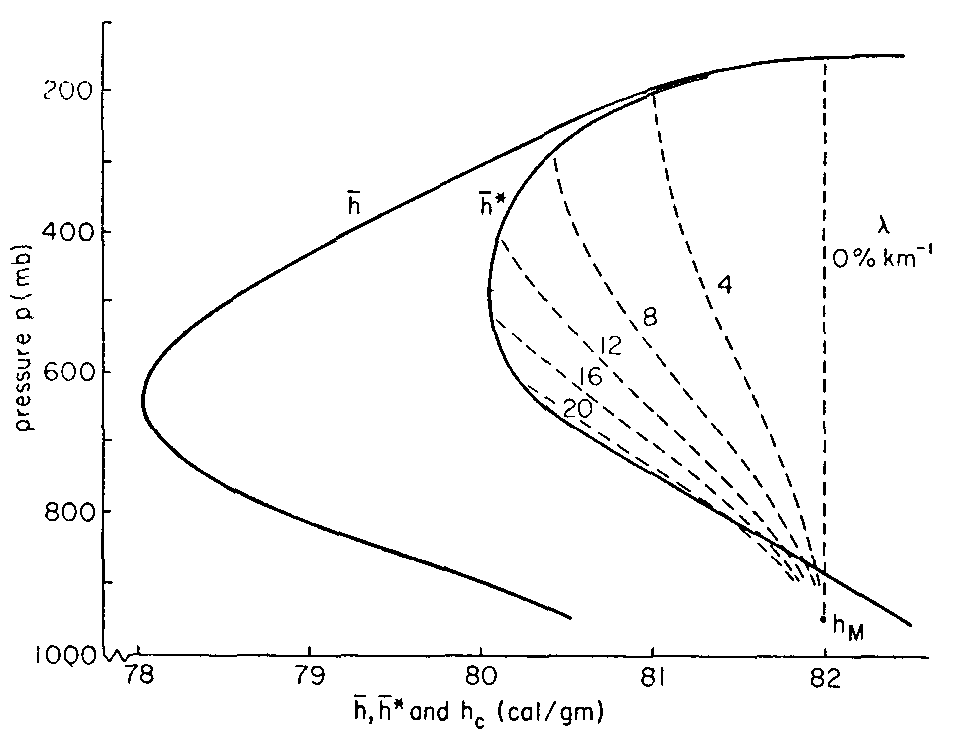
\includegraphics[height=37mm]{assets/arakawa1974/fig6.png}\hfill
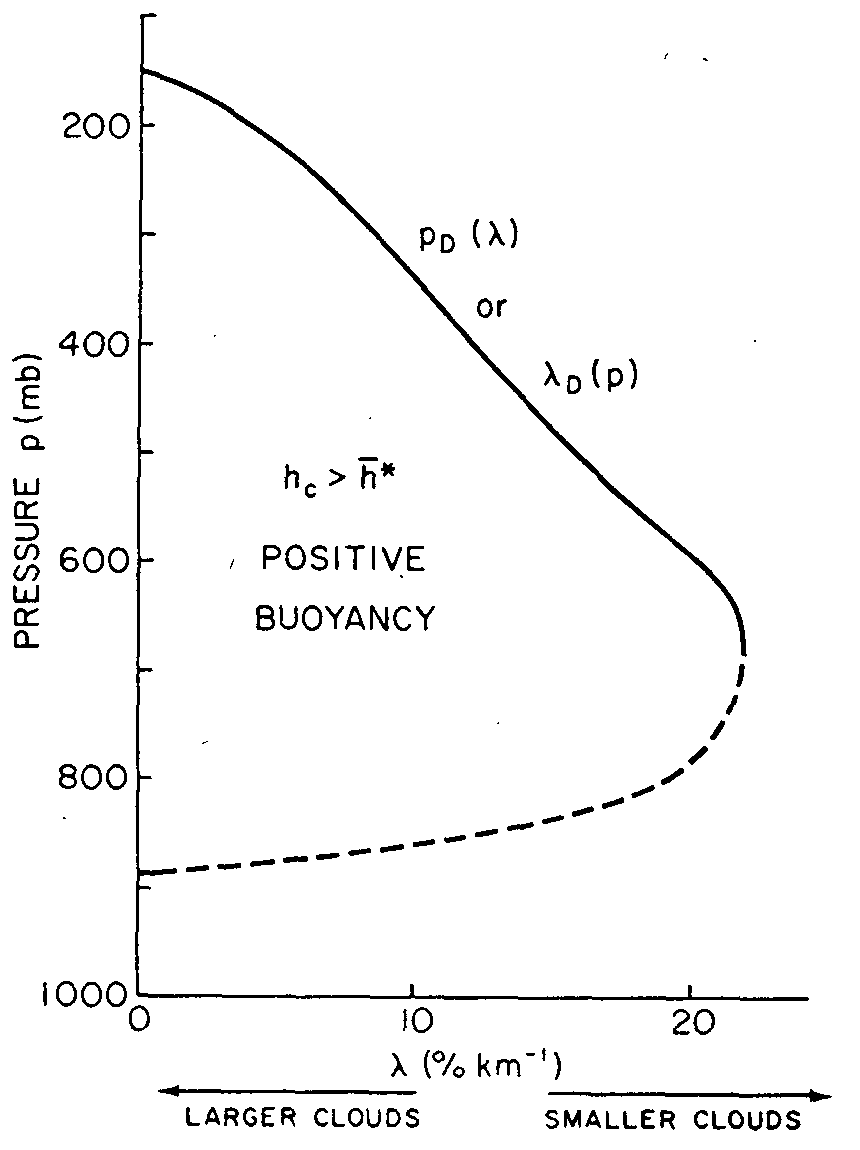
\includegraphics[height=37mm]{assets/arakawa1974/fig8.png}\hfill
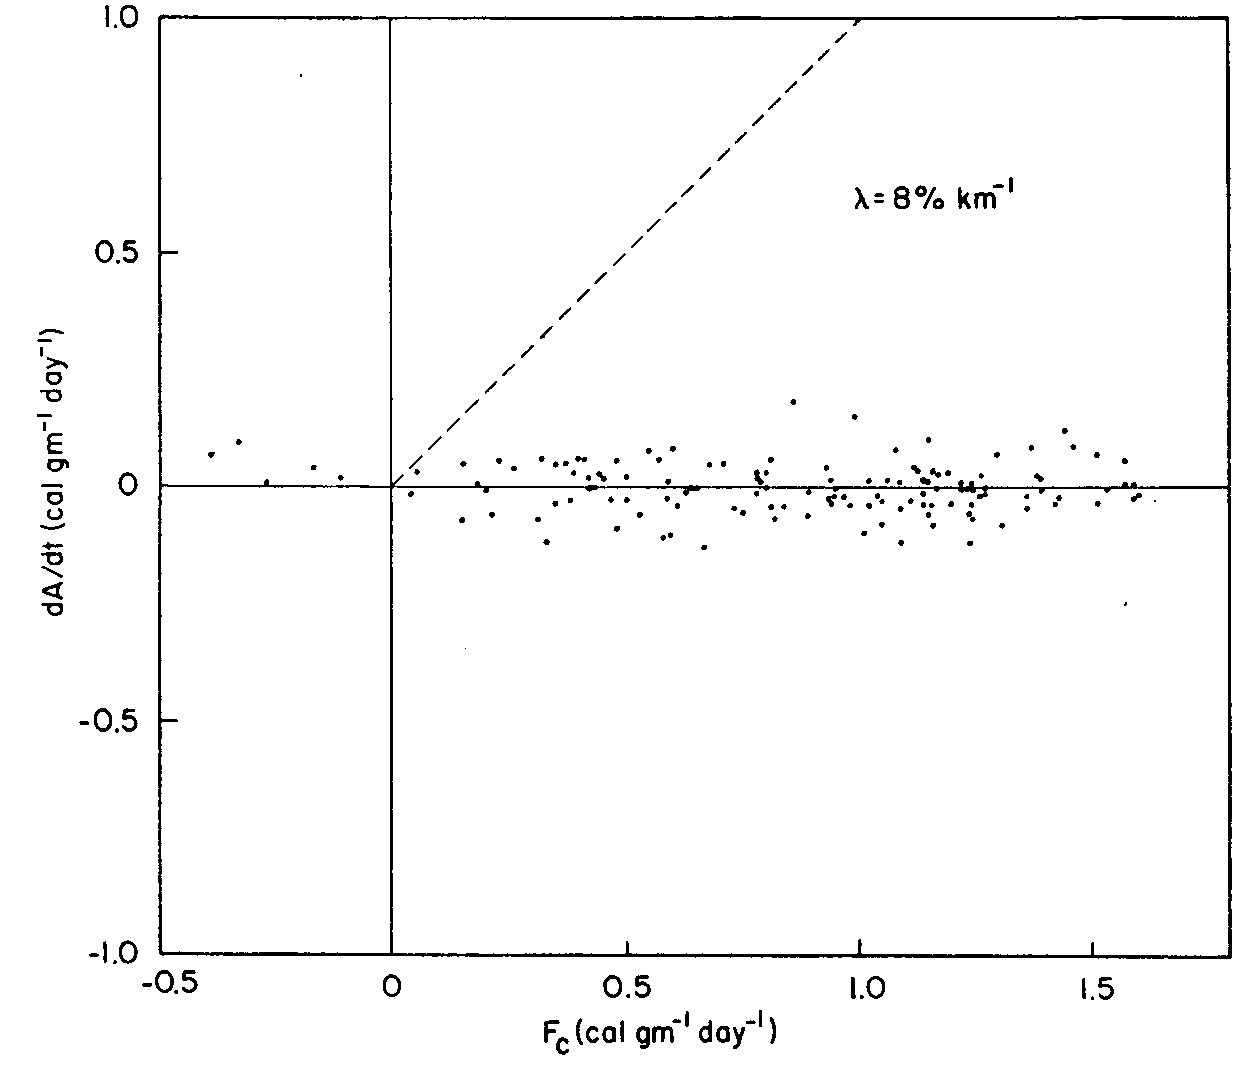
\includegraphics[height=37mm]{assets/arakawa1974/fig13a.png}\hfill
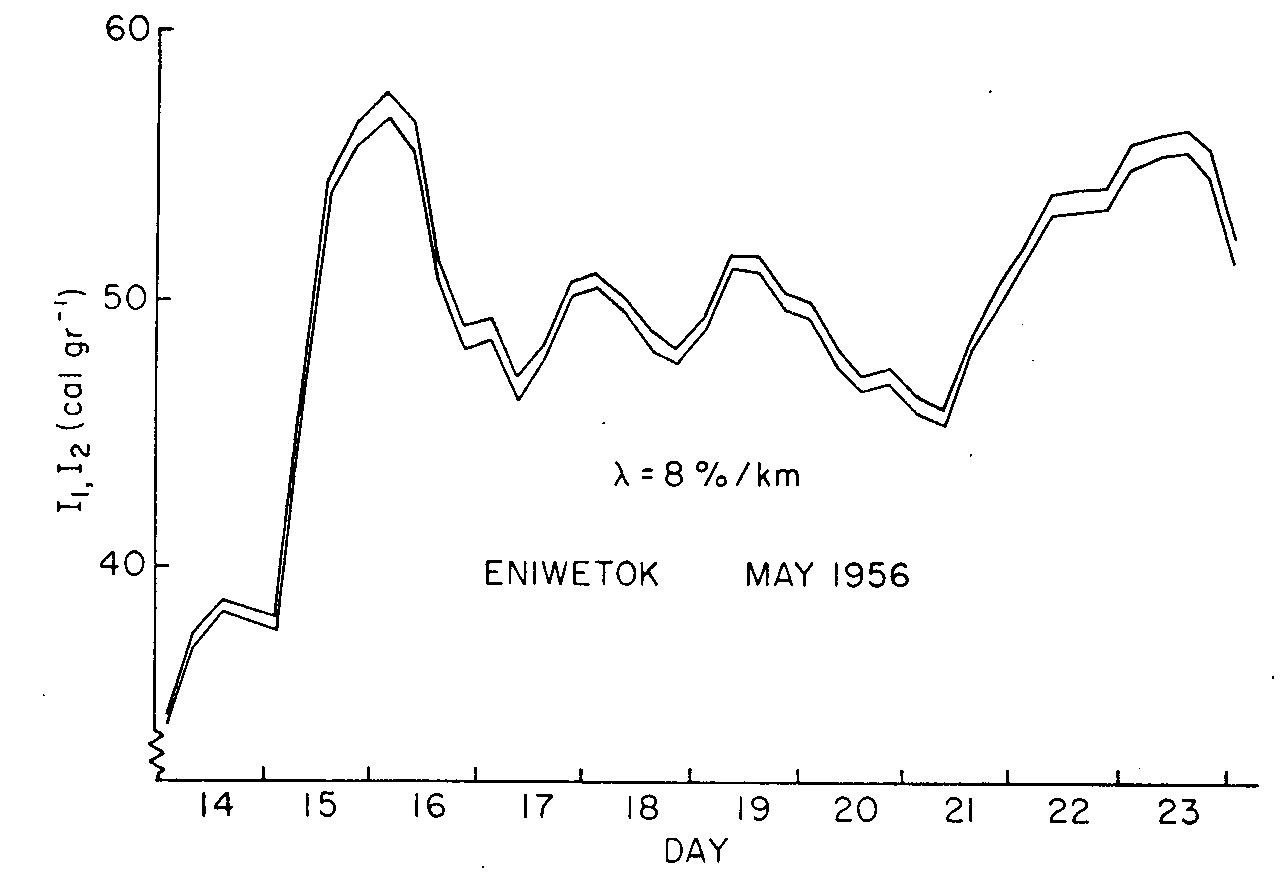
\includegraphics[height=37mm]{assets/arakawa1974/fig14.png}\par\smallskip
\begin{minipage}{\linewidth}\footnotesize\color{muted}
From left: Fig.\ 6, $\bar h$, $\bar h^*$ and $h_c(p,\lambda)$ (dashed, $\lambda$ in \% km$^{-1}$) for the mean hurricane-season sounding; Fig.\ 8, detrainment level $p_D(\lambda)$, with smaller clouds (larger $\lambda$) detraining lower; Fig.\ 13 (top panel), observed $dA/dt$ against $F_C$ for $\lambda=8\%$ km$^{-1}$, dashed line $dA/dt=F_C$; Fig.\ 14, $I_1$ and $I_2$ at Eniwetok, May 1956, whose small difference is $A$. Figures reproduced from the paper.
\end{minipage}
\end{center}
\end{document}
